\chapter{Evaluación del sistema}
\label{cap:experimentos}

Con el sistema construido resta someterlo a evaluaciones. En especial se evaluará el sistema de detección de necesidades, pues es el corazón del sistema y ha de operar con un flujo de datos constante.

\section{Topología y replicación}
\label{sec:topYPar}

En la sección \ref{subsec:topologiaSistema} se explicitó cómo estarían dispuestos los operadores en la topología, pero se ha de recordar que el sistema está pensado para operar en casos de emergencia y ha de ser capáz de escalar de acuerdo a las necesidades de la situación.\\

\textit{Apache Storm} es capaz de realizar lo anterior, pero se ha de especificar el máximo número de nodos que tendrá un nivel de operadores. Para explicar lo anterior se utilizarán las figuras \ref{fig:Implementacion1} y \ref{fig:Implementacion1p2} que muestran la implementación del la topología y una esquematización de cómo funcionaría en la peor situación, es decir, cuando el sistema determine que el nivel de replicación debería ser máximo.

\begin{figure}[H]
	\centering
	\captionsetup{justification=centering}
	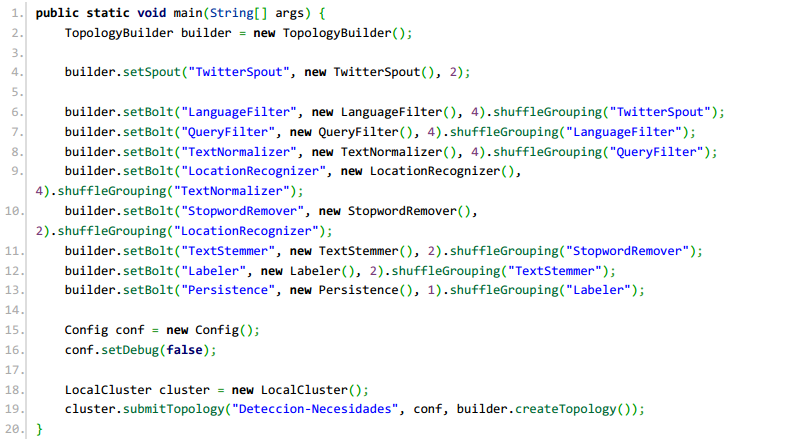
\includegraphics[scale=0.8]{images/ImplementacionTopologia1.png}
	\caption[Implementación topología de detección de necesidades.]{Implementación topología de detección de necesidades.}
	\label{fig:Implementacion1}
\end{figure}

Cada elemento de procesamiento, \textit{bolt}, es instanciado, el valor que acompaña a cada uno de ellos es el numero máximo de nodos que tendrá el sistema y seguido del modo de agrupamiento, en este caso, \textit{shuffle grouping} para balancear la carga en cada nodo.

\begin{figure}[H]
	\centering
	\captionsetup{justification=centering}
	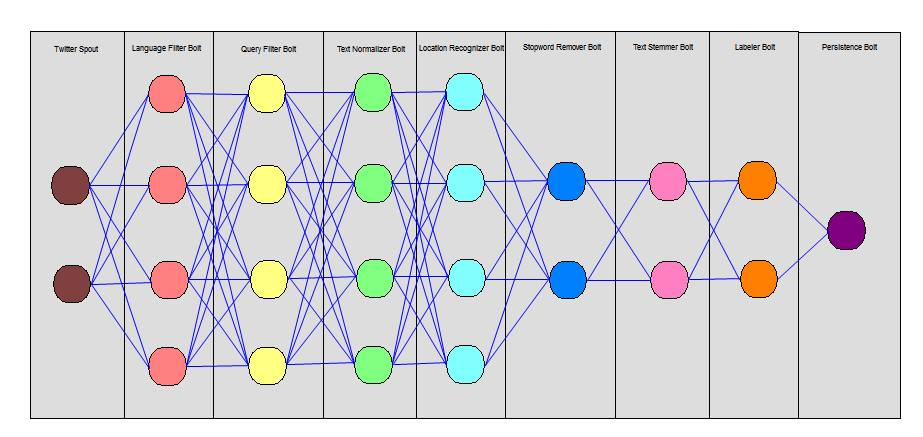
\includegraphics[scale=0.5]{images/ImplementacionTopologia1.2.png}
	\caption[Esquema de la topología en el caso de máxima actividad.]{Esquema de la topología en el caso de máxima actividad.}
	\label{fig:Implementacion1p2}
\end{figure}

Cada línea de este esquema señala comunicación de izquierda a derecha. En el caso de que el sistema trabaje al máximo de su capacidad cada nodo enviará, \textit{round robin}, estados al siguiente nivel.\\

Esta implementación y diagrama reflejan la solución inicial la cual fue decidida arbitrariamente para probar el sistema.\\

Tempranamente se detectó que el hecho de tener dos \textit{spout} resultaba contraproducente, pues enviaba, en repetidas ocaciones, el mismo estado al sistema, es decir, cuando el \textit{spout} A enviaba el estado $e_{0}$, probablemente el \textit{spout} B enviase el mismo estado $e_{0}$. Por ello se decidió eliminar el segundo \textit{spout} y limitarlo sólo a uno.\\

Se utilizó el tiempo de ejecución para 1000, 2000, 4000 y 8000 estados, pertenecientes al terremoto de Concepción el año 2010 para seleccionar cuán numeroso debería ser un nivel de nodos. Sus resultados son expuestos en la tabla \ref{tab:estadisticas}.

\begin{table}[H]
\centering
\caption{Estadísticas de los operadores para 1000, 2000, 4000 y 8000 estados}
\label{tab:estadisticas}
\begin{tabular}{|c|c|c|c|c|c|}
\hline
\multirow{2}{*}{\textbf{\begin{tabular}[c]{@{}c@{}}Entradas \\ (estados)\end{tabular}}} & \multirow{2}{*}{\textbf{Métricas}}                              & \multicolumn{4}{c|}{\textbf{Operadores}}                                         \\ \cline{3-6} 
                                                                                        &                                                                 & \textbf{Idioma} & \textbf{Normalizador} & \textbf{Ubicación} & \textbf{Stopword} \\ \hline
\multirow{4}{*}{\textbf{1000}}                                                          & \textbf{Procesados}                                             & 1000            & 1000                  & 1000               & 1000              \\ \cline{2-6} 
                                                                                        & \textbf{Emitidos}                                               & 402 (40.20\%)   & 1000 (100\%)          & 623 (62.30\%)      & 1000 (100\%)      \\ \cline{2-6} 
                                                                                        & \textbf{Descartados}                                            & 598 (59.80\%)   & 0 (0\%)               & 377 (37.70\%)      & 0 (0\%)           \\ \cline{2-6} 
                                                                                        & \textbf{\begin{tabular}[c]{@{}c@{}}Tiempo \\ (ms)\end{tabular}} & 513             & 28999                 & 1713114            & 38064             \\ \hline
\multirow{4}{*}{\textbf{2000}}                                                          & \textbf{Procesados}                                             & 2000            & 2000                  & 2000               & 2000              \\ \cline{2-6} 
                                                                                        & \textbf{Emitidos}                                               & 807 (40.35\%)   & 2000 (100\%)          & 1058 (52.90\%)     & 2000 (100\%)      \\ \cline{2-6} 
                                                                                        & \textbf{Descartados}                                            & 1193 (59.65\%)  & 0 (0\%)               & 942 (47.10\%)      & 0 (0\%)           \\ \cline{2-6} 
                                                                                        & \textbf{\begin{tabular}[c]{@{}c@{}}Tiempo\\ (ms)\end{tabular}}  & 908             & 77259                 & 1415104            & 46093             \\ \hline
\multirow{4}{*}{\textbf{4000}}                                                          & \textbf{Procesados}                                             & 4000            & 4000                  & 4000               & 4000              \\ \cline{2-6} 
                                                                                        & \textbf{Emitidos}                                               & 1673 (41.83\%)  & 4000 (100\%)          & 1985 (49.63\%)     & 4000 (100\%)      \\ \cline{2-6} 
                                                                                        & \textbf{Descartados}                                            & 2327 (58.17\%)  & 0 (0\%)               & 2015 (50.37\%)     & 0 (0\%)           \\ \cline{2-6} 
                                                                                        & \textbf{\begin{tabular}[c]{@{}c@{}}Tiempo\\ (ms)\end{tabular}}  & 1657            & 47225                 & 2437992            & 63437             \\ \hline
\multirow{4}{*}{\textbf{8000}}                                                          & \textbf{Procesados}                                             & 8000            & 8000                  & 8000               & 8000              \\ \cline{2-6} 
                                                                                        & \textbf{Emitidos}                                               & 3101 (38.76\%)  & 8000 (100\%)          & 4113 (51.41\%)     & 8000 (100\%)      \\ \cline{2-6} 
                                                                                        & \textbf{Descartados}                                            & 4899 (61.24\%)  & 0 (\%)                & 3887 (48.59\%)     & 0 (0\%)           \\ \cline{2-6} 
                                                                                        & \textbf{\begin{tabular}[c]{@{}c@{}}Tiempo\\ (ms)\end{tabular}}  & 3658            & 55311                 & 4681626            & 92825             \\ \hline
\end{tabular}
\end{table}

Con estos resultados se busca definir los balores para la cantidad de nodos por cada nivel de bolts, de la tabla podemos concluir lo siguiente:

\begin{itemize}
\item En relación al normalizador, eliminador y stemmer (no se incluyó en la tabla pues su comportamiento es idéntico a las dos anteriores), la entrada y salida es 1 a 1, es decir, por cada elemento que entra, saldrá un elemento. Por ello, y para no originar cuellos de botella, tendrán la misma cantidad de nodos que el \textit{bolt} anterior. 
\item Para un aumento exponencial de datos, el filtro de idioma es, aproximadamente, constante en permitir el paso del 40\% de los estados. Esto quiere decir que el filtro siguiente, debería contener el 40\% de los \textit{bolts} del filtro de idioma.
\item Para un aumento exponencial de datos, el filtro por ubicación, aproximadamente, permite el paso del 50\% de los datos. Es decir, el \textit{bolt} siguiente debería tener el 50\% de los nodos que tiene el nivel de ubicación.
\item El tiempo de ejecución del filtro de ubicación es el más alto de todos, debido a ello pueden producirse cuellos de botella, es recomendable, entonces, aumentar el número de elementos de procesamiento.
\item 
\end{itemize}

En función de lo anterior, y tomando como solución inicial lo expuesto en la figura \ref{fig:Implementacion1p2} la configuración de la topología del detector de necesidades quedaría de la siguiente forma:

\begin{enumerate}
\item \textit{Spout Twitter}: 1 nodo.
\item \textit{Bolt} Idioma: 4 nodos.
\item \textit{Bolt} Filtro de Consultas: 2 nodos.
\item \textit{Bolt} Normalizador: 2 nodos.
\item \textit{Bolt} Ubicación: 2 nodos.
\item \textit{Bolt Stopword}: 1 nodo.
\item \textit{Bolt Stemmer}: 1 nodo.
\item \textit{Bolt} Etiquetador: 1 nodo.
\item \textit{Bolt} Persistencia: 1 nodo.
\end{enumerate}

\section{Funcionamiento en alto tráfico}
\label{sec:AltoTrafico}

